\section{Theory}

Raman spectroscopy uses the interactions between the analyte and incident electromagnetic radiation to determine its characteristic vibrations. These characteristic vibrations can be used to draw conclusions about the structure of a molecule, and in reverse, knowing the structure of a molecule one can predict its Raman spectrum. 
\bigskip

A peak in the raman spectrum of a molecule appears if the polarizability \( \alpha \) of a bond changes as a result of the interaction between the photon and the molecule. This means that not all bonds and vibrational modes appear in a Raman spectrum. 

\bigskip

There are three kinds of scattering, Rayleigh scattering, where the wavelength of the scattered photon is the same as the excitation photon, Stokes scattering, where the wavelength is lower, and Anti-Stokes scattering, where the wavelength is higher. It is experimentally proven that much less photons undergo Anti-Stokes scattering than Stokes scattering.
First, the phenomenon will be described using classical mechanics, later a quantum-mechanical explanation will be added. 


\subsection{Light and Matter}

According to classical theory, an oscillating electric dipole is the most efficient source of electromagnetic radiation. Thus we must consider the distribution of electric charges within the molecule in order to understand the origin of the scattered light. We must establish whether there is an electric dipole, permanent or induced, which when modulated by the normal vibrations, could oscillate.

\bigskip
An electric dipole of the form: two charges, \(+q\) and \(-q\) separated by a distance \(r\), is defined by its dipole moment \(\mu\), defined as:
\begin{equation}
    \mu=qs
\end{equation}

\(\mu\): dipole moment (\unit{\coulomb\meter})\\
\(q\): charge (\unit{\coulomb})\\
\(s\): vector pointing from \(-q\) to \(+q\) (\unit{\meter})

If such a dipole oscillates with a frequency \(\nu\), which corresponds to the wavelenth \(\widetilde{\nu}=\frac{\nu}{c}\), \(c\) being the speed of light, then it emits electromagnetic radiation of the same wavelength.

\bigskip

In a polyatomic molecule, a permanent electric dipole moment is formed when the center of positive charges and the center of negative charges do not coincide. Regardless of whether the molecule has a permanent electric dipole moment, it might change as nuclei are moved from their equilibrium positions due to normal vibrations. Since the changes are periodic in time, for a frequency \(\nu_k\) of a given normal vibration, 

\begin{equation}
    \mu=\mu_0cos(2\pi\nu_kt)
\end{equation}

\(\mu\): change of the instantaneous dipole moment from the permanent dipole moment(\unit{\coulomb\meter})
\(\nu_k\): frequency of a normal vibration (\unit{\hertz})\\
\(\mu_0\): amplitude of the dipole moment (\unit{\coulomb\meter})

\bigskip

This oscilating dipole moment is capable of absorbing and emitting light with the frequency \(\nu_k\).
Scattering of light by a molecule is associated with oscillations of an induced electric dipole. An external electric field will polarize the molecule, creating an induced electric dipole. If this induced dipole oscillates, it can produce electromagnetic radiation. If the external electric field is static, the only possible frequencies are the ones of the normal vibrations of the molecule, while if the electric field oscillates, for example like a beam of light,the induced dipole follows the alternating electric field while also being modulated by the normal vibrations of the nuclei. This results in it oscillating in combinations of the frequencies of the external electric fiels and the normal vibration, radiation all those frequencies. \cite{theory1}

\subsection{Classical Description}


The classical theory of Rayleigh and Raman scattering is based on the concept that incident radiation, an electromagnetic wave, has an electric field which induces an oscillating dipole moment which generates scattered light. The following power series describer the relation between the induced dipole moment vector \(\overrightarrow{\mu} \) and the electric field vector \(\overrightarrow{E} \): 

\begin{equation} \label{eq:vectors_power_series}
    \overrightarrow{\mu} = \alpha \overrightarrow{E} + \frac{1}{2} \beta \overrightarrow{E}\overrightarrow{E} + \frac{1}{6} \gamma \overrightarrow{E}\overrightarrow{E}\overrightarrow{E} + \dots
\end{equation}

\(\overrightarrow{\mu} \): induced dipole moment vector (\unit{\coulomb\meter})\\
\(\overrightarrow{E} \): electric field vector (\unit{\volt\per\meter})\\
\(\alpha\): polarizability (\unit{\coulomb\meter\squared\per\volt}) \\
\(\beta\): hyperpolarizability (\unit{\coulomb\meter\cubed\per\volt\squared}) \\
\(\gamma\): second hyperpolarizability (\unit{\coulomb\meter^4\volt^{-3}}) 

\bigskip

Polarizabilities \( \alpha, \beta\) and \( \gamma\) are tensors of rank 2,3 and 4 respectively. They describe physical properties responsible for the connections between vectorial quantities and are typically represented by matrixes. A tensor of rank n can be represented by an n-dimentional matris. The tensor of rank 2 can be written as a 3x3 matrix. The polarizability describes a molecules tendency to develop a dipole moment when in an electric field, the flexibility of the molecules electron cloud. The non-linear terms in Equation \ref{eq:vectors_power_series} are usually very small when compared to the linear term and do not play a role in normal, linear Raman scattering. By restricting Equation \ref{eq:vectors_power_series} to it's linear component, i.e.


\begin{equation} \label{eq:vectors_power_series_lin}
    \overrightarrow{\mu} = \alpha \overrightarrow{E}
\end{equation}

it can be written in the form of three linear equations correspnding to a matrix multiplication

\begin{equation}
    \begin{bmatrix}
        \mu_x\\
        \mu_y\\
        \mu_z\\
    \end{bmatrix}
    = 
    \begin{bmatrix}
        \alpha_{xx} & \alpha_{xy} & \alpha_{xz} \\
        \alpha_{yx} & \alpha_{yy} & \alpha_{yz}\\
        \alpha_{zx} & \alpha_{zy} & \alpha_{zz}\\
    \end{bmatrix}
    \begin{bmatrix}
        E_x\\
        E_y\\
        E_z\\
    \end{bmatrix}
\end{equation}

where the nine coefficients \(\alpha_{ij} \) are components of the polarizability tensor \(\alpha\). X, Y and Z refer to the axes of the chosen coordienate system. Some important properties of this and similar tensor keys will briefly be described.

\bigskip

The polarizability tensor can be described by a real, symmetric matrix where \(\alpha_{ij} = \alpha_{ji}\). This matrix is only necessarily symmetric for nonresonant Raman spectroscopy. 

\bigskip

The polarizability tensor of a molecule can be graphically represented by an ellipsoid with usually three different half-axes. Its shape is independent of the chosen reference coordinate system, but the actual values of the chosen tensor components will differ based on the chosen orientation of axes. If the axes of reference coincide with the principal axes of the polarizability ellipsoid, all off-diagonal elements of the polarizability tensor vanish and a simpler,  diagonal matrix remains. While the individual components change, there are certain invariants, one being the mean variance \(\alpha\), defined as the average of \(\alpha_{xx}, \alpha_{yy} \) and \(\alpha_{zz}\):

\begin{equation}
    \alpha=\frac{1}{3}(\alpha_{xx}+\alpha_{yy}+\alpha_{zz})
\end{equation}

\bigskip


The polarizability \(\alpha\) is a continuous function of the nuclear displacement \(q_k\) for the k-th normal vibrational mode, and as such can be expanded into a Taylor series:

\begin{equation} \label{eq:polarizability}
    \alpha=\alpha_{q=0} + 
    \left( \frac{\partial\alpha}{\partial q_k}\right)_{q=0}q + highter\:order\:terms
\end{equation}



As the displacement q is small, the higher order terms, which would account for non-linear effects, can be ignored. 

\bigskip

The electric field produced by the electromagnetic wave with frequency \(\nu_0\) interacts with the molecule and forces a change in polarizability, which results in an induced dipole moment \(\mu\).

\begin{equation} \label{eq:electic_field}
    E = E_0cos(2\pi\nu_0t)
\end{equation}

\(E\): electric field at time t (\unit{\volt\per\meter})\\
\(E_0\): maximal electric field (\unit{\volt\per\meter})\\
\(\nu_0\): frequency electromagnetic wave (\unit{\hertz}) \\
\(t\): time at which the electric field is calculated (\unit{\second})

\begin{equation} \label{eq:dipole_moment}
    \mu = \alpha E
\end{equation}

\(\mu\): dipole moment (\unit{\coulomb\meter}) \\
\(\alpha \): polarizability 
(\unit{\coulomb\meter\squared\per\volt})\\


The polarizability describes a molecules tendency to develop a dipole moment when in an electric field. This would of course depend on the distance between the nuclei of the molecule, which fluctuates as the bond vibrates. As such it can be written as a function of the nuclear displacement \(q\) with \(q_0=\)maximum displacement.

\begin{equation} \label{eq:nuclear_displacement}
   q=q_0cos(2\pi\nu_kt)
\end{equation}

\(q\): nuclear displacement at time t (\unit{\meter}, but for molecular vibrations \unit{\angstrom} is used sometimes)\\
\(q_0\): amplitude, maximum diplacement (\unit{\meter}, but for molecular vibrations \unit{\angstrom} is used sometimes)\\
\(\nu_k \) : frequency k-th internal vibration (\unit{\hertz}) \\
\(t\): time at which the displacement is calculated (\unit{\second})


\bigskip 

Substituting Equations \ref{eq:electic_field}, \ref{eq:nuclear_displacement} and \ref{eq:polarizability} into Equation \ref{eq:dipole_moment} and expanding it using trigonometric identities results in:

\begin{multline} \label{eq:dipole_moment_expanded}
    \mu = (\alpha_{q=0} + \left( \frac{\partial\alpha}{\partial q_k}\right)_{q=0}q)*E_0cos(2\pi\nu_0t) = \\
    = \alpha_{q=0}*E_0cos(2\pi\nu_0t) +  \left( \frac{\partial\alpha}{\partial q_k}\right)_{q=0}q_0*cos(2\pi\nu_kt)*E_0cos(2\pi\nu_0t)=\\
    =\alpha_{q=0}*E_0cos(2\pi\nu_0t) + \frac{1}{2} \left( \frac{\partial\alpha}{\partial q_k}\right)_{q=0}q_0E_0\left(cos(2\pi(\nu_0-\nu_k)t)+cos(2\pi(\nu_0-\nu_k)t)\right)= \\
    =\alpha_{q=0}*E_0cos(2\pi\nu_0t)+\frac{1}{2} \left( \frac{\partial\alpha}{\partial q_k}\right)_{q=0}q_0E_0cos(2\pi(\nu_0-\nu_k)t) + \frac{1}{2} \left( \frac{\partial\alpha}{\partial q_k}\right)_{q=0}q_0E_0cos(2\pi(\nu_0+\nu_k)t)
\end{multline}

The different arguments of the three cosine functions mean that the molecule oscillates with three distinct frequencies simultaneously, each corresponding to three different emitted frequencies of light, \(\nu_0\), \(\nu_0-\nu_k\) and \(\nu_0+\nu_k\). They correspond to Rayleigh scattering, where the frequency of the photon stays the same, Stokes scattering, where the scattered photon has a lower frequency, and Anti-Stokes scattering, where the scattered photon has a higher frequency.

\bigskip

Equation \ref{eq:dipole_moment_expanded} also shows that Stokes and Anti-Stokes scattering only appears if \((\frac{\partial\alpha}{\partial q})_{q=0}\neq 0\), which means that in order for a vibrational mode to be raman active, the vibrational mode has to change the polarizability.

\bigskip

Equation \ref{eq:dipole_moment_expanded} implies that Stokes and Anti-Stokes scattering have the same intensity, which has been proven to be wrong experimentally. For example Figure \ref{fig:dcm_i}, an experimentally aquired Raman spectrum of dichloromethane where the Rayleigh scattering has been removed and the difference of the recorded wavelengths to the excitation wavelength has been calculated in terms of wavenumber, which is the reciprocal of the wavelength, shows clearly that the scattering is not symmetric, it is clearly much higher on one side. This makes it clear that a purely classical mechanical approach is not enough to explain this phenomenon and a quantum mechanical approach is needed. \cite{theory1} \cite{presentation}

\bigskip

An N-atomic molecule has 3N degrees of freedom: each atom has 3 translational coodrinates. 3 of those 3N degrees of freedom correspond to translational degrees of freedom, moving the whole molecule in some direction. 3 (resp. 2 for linear molecules) of the remaining 3N-3 degrees of freedom corrsepond to rotational degrees of freedom, which means that an N-atomic molecule has 3N-6 (resp. 3N-5) vibrational degrees of freedom. \cite{molecularvibration}

\newpage

\subsection{Quantum Mechanical Approach}

The basic principles of quantum dynamics state that energy associated with vibrational, rotational and electronic degrees of freedom of a molecule can assume values only from a discrete set. This set contains the quantized energy levels corresponding to the possible stationary states of the molecule.

\begin{figure}[h]
    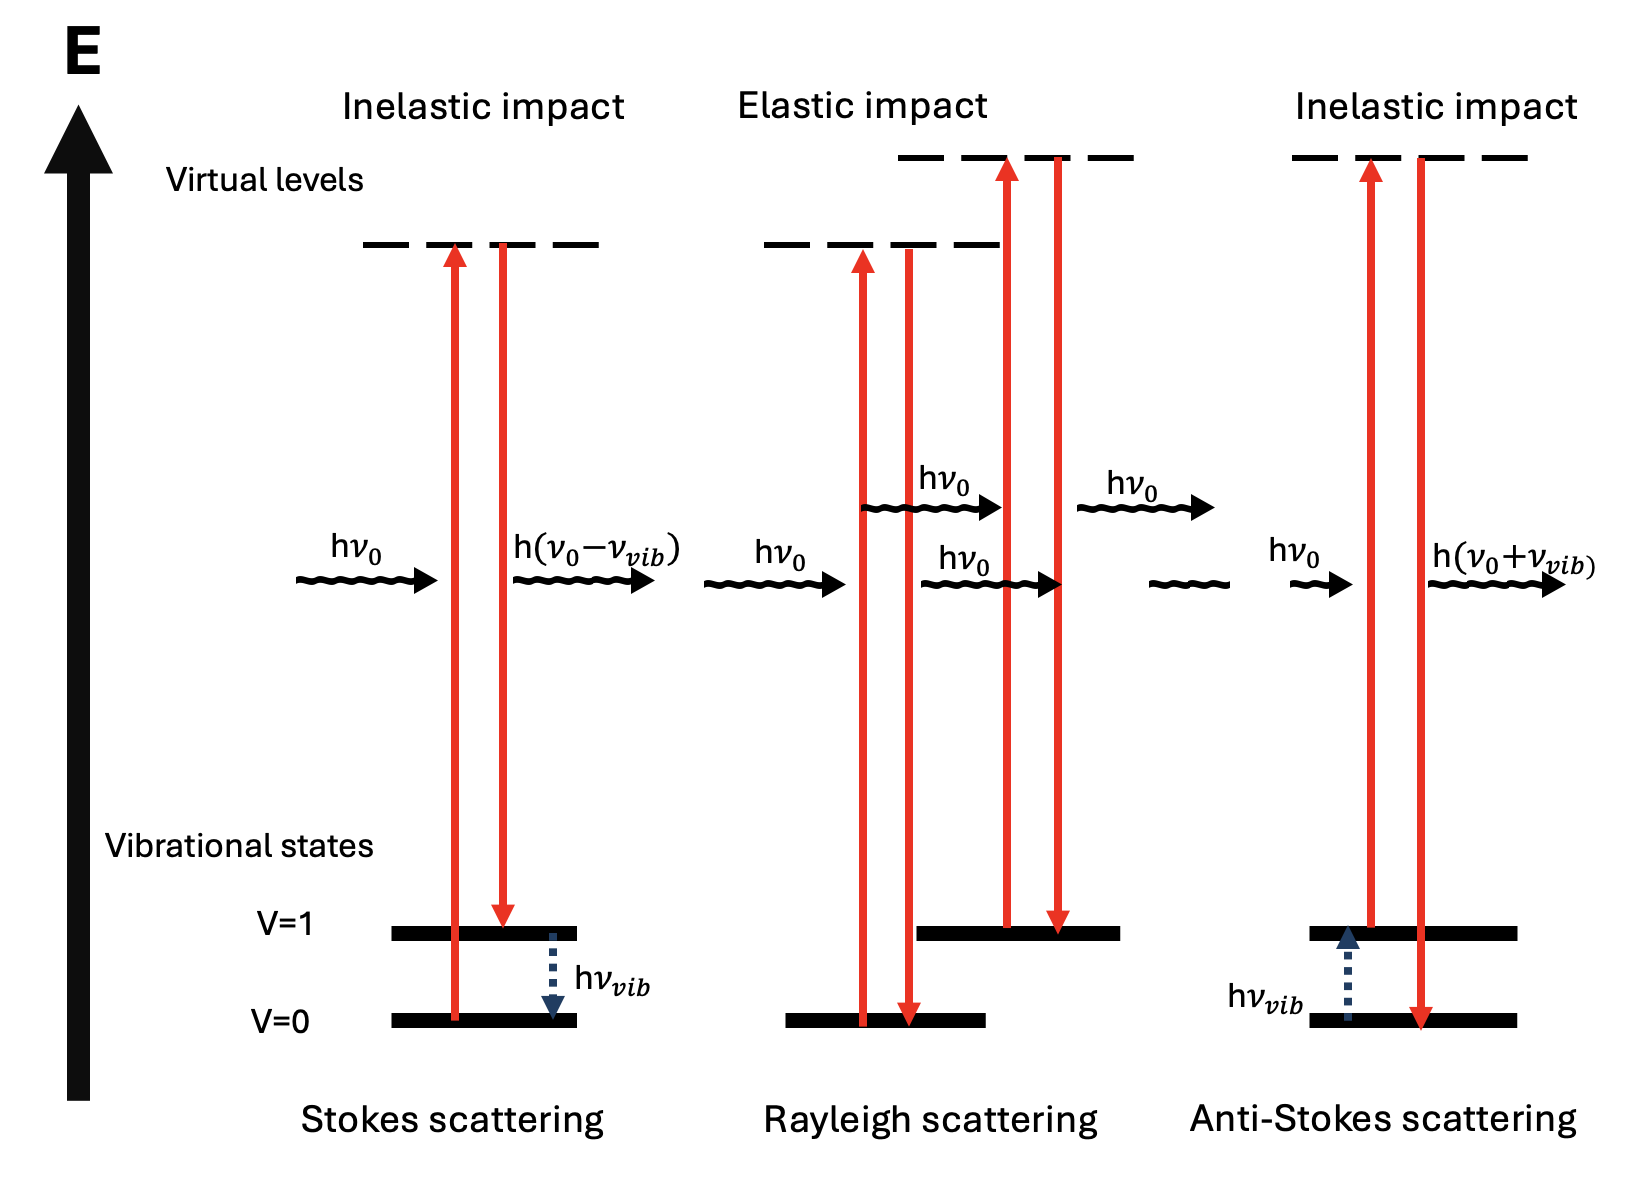
\includegraphics[width=\textwidth]{images/theory/qm_scattering.png}
    \caption{6. Diagram of transitions between vibrational energy levels corresponding to the processes of Rayleigh and Raman scattering.}
    \label{fig:energy_model}
\end{figure}

In quantum mechanics, absorbtion and emission of radiation by a molecular system are results of upward resp. downward transitions between two energy levels. The radiation absorbed resp. emitted is quantized, the energy enclosed in disctrete photons that can be viewed as electromagnetic waves. The change in energy of the molecule, \(\pm\Delta E\), is equivalent to the energy of the photon emitted or absorbed (Figure \ref{fig:energy_model}). The energy \(E\) of a photon is directly proportional to its frequency:

\begin{equation}
    E = h \nu
\end{equation}

\( E\): energy of a photon (\unit{\joule})\\
\( h\): Planck's constant (\SI{6.62608e-34}{\joule\second})\\
\(\nu\): frequency of the photon (\unit{hertz})

\bigskip

Rayleigh and Raman scattering invorve two transitions which occur at almost the same time: one photon of the incident radiation is annihilated and the molecule transitions into a virtual state, and another photon, either of the same energy (Rayleigh scattering), lower energy (Stokes scattering) or higher energy (Anti-Stokes scattering) is created. The virtual state is a transition state which is not one of the eigenstates of the molecule, so it is only imaginary and used to separate the energy transition into two one-photon processes. 

\bigskip

Quantum mechanics also explains the discreptancy between 
 the intensities of the Stokes and Anti-Stokes scattering. In order to undergo Anti-Stokes scattering, the molecule has to be on an energy level which it can fall down from. At room temperature, most molecules are in their lowest energy level, which means that only a few are capable of Anti-Stokes scattering. The equilibrium of the population of the states is giveb my the Boltzmann thermal distribution:

 \begin{equation}
    \frac{N_i}{N_j} = exp \left( \frac{E_j-E_i}{kT}\right)
 \end{equation}

\(N_i\): population state i \\
\(N_j\): population state j \\
\(E_i\): energy state i (\unit{\joule})\\
\(E_j\): energy state j (\unit{\joule})\\
\(k\): Boltzmann constant (\SI{1.380649e-23}{\joule\per\kelvin})\\
\(T\): temperature of the system (\unit{\kelvin})

\bigskip

The relative intensities of the Stokes and Anti-Stokes scattering is given by:

\begin{equation}
    \frac{I_{Stokes}}{I_{Anti-Stokes}} = \frac{I_{\widetilde{\nu_0} - \widetilde{\nu_k}}}{I_{\widetilde{\nu_0} + \widetilde{\nu_k}}} = \frac{(\widetilde{\nu_0} - \widetilde{\nu_k})^4}{(\widetilde{\nu_0} + \widetilde{\nu_k})^4}exp \left( \frac{hc\widetilde{\nu_k}}{kT}\right)
 \end{equation}

 \(I_{Stokes}\): intensity Stokes scattering (\unit{\watt})\\
 \(I_{Anti-Stokes}\): intensity Anti-Stokes scattering (\unit{\watt})\\
\(\widetilde{\nu_0}\): wavenumber incident light (cm\(^{-1}\))\\
\(\widetilde{\nu_k}\): wavenumber corresponding to the energy difference between states (cm\(^{-1}\))\\
\( h\): Planck's constant (\SI{6.62608e-34}{\joule\second})\\
\(c\): speed of light (\SI{2.99792458e8}{\meter\per\second})\\
\(k\): Boltzmann constant (\SI{1.380649e-23}{\joule\per\kelvin})\\
\(T\): temperature of the system (\unit{\kelvin})

\bigskip


which explains the discreptancy that is made by the classical mechanical approach. \cite{theory1} \cite{presentation}

\newpage

\subsection{Group Theory}
The mathematical group theory can be used to describe multi-atomic molecules in order to predict, describe and classify many molecular properties. In the case of Raman spectroscopy, group theory is used to predict the number of raman bands of a molecule as well as a qualitative description of the normal modes of vibration with which they are associated.

\bigskip

Group theory can be used to conduct structural analyses of raman active compuonds. The symmetry of a molecule determines whether a vibration is raman active. 

\bigskip

In a molecule, a movement from one position to another one which is indistinguishable from the original one is called a symmetry operation. Each symmetry operation is carried out with respect to a geometric entity, be it a plane, a line or a point, which is called a symmetry element. There is a limited number of possible symmetry elements. Molecules can have one or more symmetry elements, although not all combinations of symmetry elements are possible. Each set of possible symmetry combinations is called a "point group". Most known molecules have lod degrees of molecular symmetry, so the number of relevant point groups is limited. For each point groups, there exist character tables which can be used to calculate the expected number of Raman active modes as well as Raman peaks. \cite{gt}